\chapter{基于说话人特征的跨语种语音转换优化方法}

\section{引言}

上文介绍了本文提出了基于半优化CycleGAN的非平行语料语音转换系统,该框架可以在一般非平行语料的语音转换任务上
得到较高的音质。然而,当原始说话人和目标说话人两个领域的差距较大时,转换的难度就会显著增加,差距可以体现在
说话人信息,语速,语义,音调等。在这种情况下,转换语音的音质会有明显的下降,甚至会无法训练。另一方面,实际
应用场景中,两个差距较大的领域是比较常见的,之前实验中的数据都是在专业录音环境下录制的平稳朗读语音,属于较为
理想的情况。因此,对领域差距较大情况下的语音转换任务进行优化具有较高的实际应用价值和研究价值。本章将对其中
较为极端的任务作为研究对象,即跨语种的语音转换。在该任务中,两个领域不仅是说话人信息不同,在语义信息上也
具有较大的差异,这对模型性能提出了挑战。

本章提出一种基于说话人特征的跨语种语音转换方法,以第三章介绍的CycleGAN-VC方法为基础,在CycleGAN模型中引入
说话人识别机制。首先需要先训练一个说话人识别模型,之后使用模型中的d-vector提取器来作为CycleGAN中判别器的
前置模型,使得判别器可以只使用说话人信息作为判别标准。实验证明,引入说话人特征的语音转换方法可以有效实现
在保留语义的前提下实现说话人语音转换,有效提升模型性能。

在接下来的内容中,将首先对跨语种语音转换和相关工作进行简要介绍,然后对说话人识别及其相关特征进行说明,
之后将详细介绍本章提出的引入说话人特征的跨语种语音转换优化方法,最后对实验配置及其结果进行分析。

\section{跨语种语音转换}
\subsection{跨语种语音转换概述}
根据转换语言条件的不同,可以将语音转换分为两类:单语种语音转换和跨语种语音转换。在单语种语音转换中,训练集中
原始说话人和目标说话人的语言是相同的,在测试时也是同一种语言。相对的,跨语种语音转换则是原始说话人和目标说话人的
语言不同,在此基础上可以将其再分为两类:一类是原始说话人的训练集是双语种的,其中一个语种和目标说话人一致;另一类
则是完全不相同。早期在跨语种语音转换上的研究多基于第一类情况,在本章我们则将以第二类为研究对象。跨语种语音转换具有较好
的发展和应用前景,作为无监督学习任务,其可以实现让一个不会说某种语言的说话人以他的声音说该语言。在语音翻译中,
通常需要将某个说话人的语音翻译为另一种语言的语音,然而翻译语音通常不是该说话人的声音,跨语种语音转换便可以作为
补充,完善语音翻译的整个环节。

尽管跨语种的语音转换的研究仍处于初步阶段,但研究人员针对跨语种的特点,提出了一些有效的方法。在\cite{AbeStatistical}中,
一个双语种的转换模型在目标语言的平行训练数据上训练,这需要原始说话人的训练数据不仅包含原始语种,也包含目标语种。
然而,事实上双语种说话人的双语数据是较难获得的。因此一些用于在非平行数据中找到对应的原始-目标帧的非平行对齐技术
被开发出来,例如单元选择\cite{sundermann2006text,Hao2015AA}和迭代对齐法\cite{erro2007frame,erro2009inca}。
但是这些方法由于不准确性使得转换性能只处于中等。基于声道长度归一化的音素映射方法也被提出\cite{sundermann2003vtln,qian2011frame},
这些方法中弯折函数是通过原始和目标特征之间最接近的音素或声学类来估计的。研究人员也提出了基于音素后验概率图的方法\cite{sun2016personalized,zhou2019cross},
该方法使用单语种或双语种的音素字典来作为中间的说话人无关特征,实现跨语种的转换。

\subsection{跨语种语音转换的难点}
% 1.不同语种之间文本信息不一致导致较难匹配
% 2.不同语种声学特征差异较大,对cyclegan有挑战性
如前文所述,跨语种语音转换作为一个无监督任务,是非平行语料语音转换的一个特殊任务。相比于通常的非平行语料语音转换,
跨语种语音转换转换难度更大,目前方法的效果也都不尽如人意。主要难度体现在以下两个方面。

\begin{figure}[!htp]
    \centering
    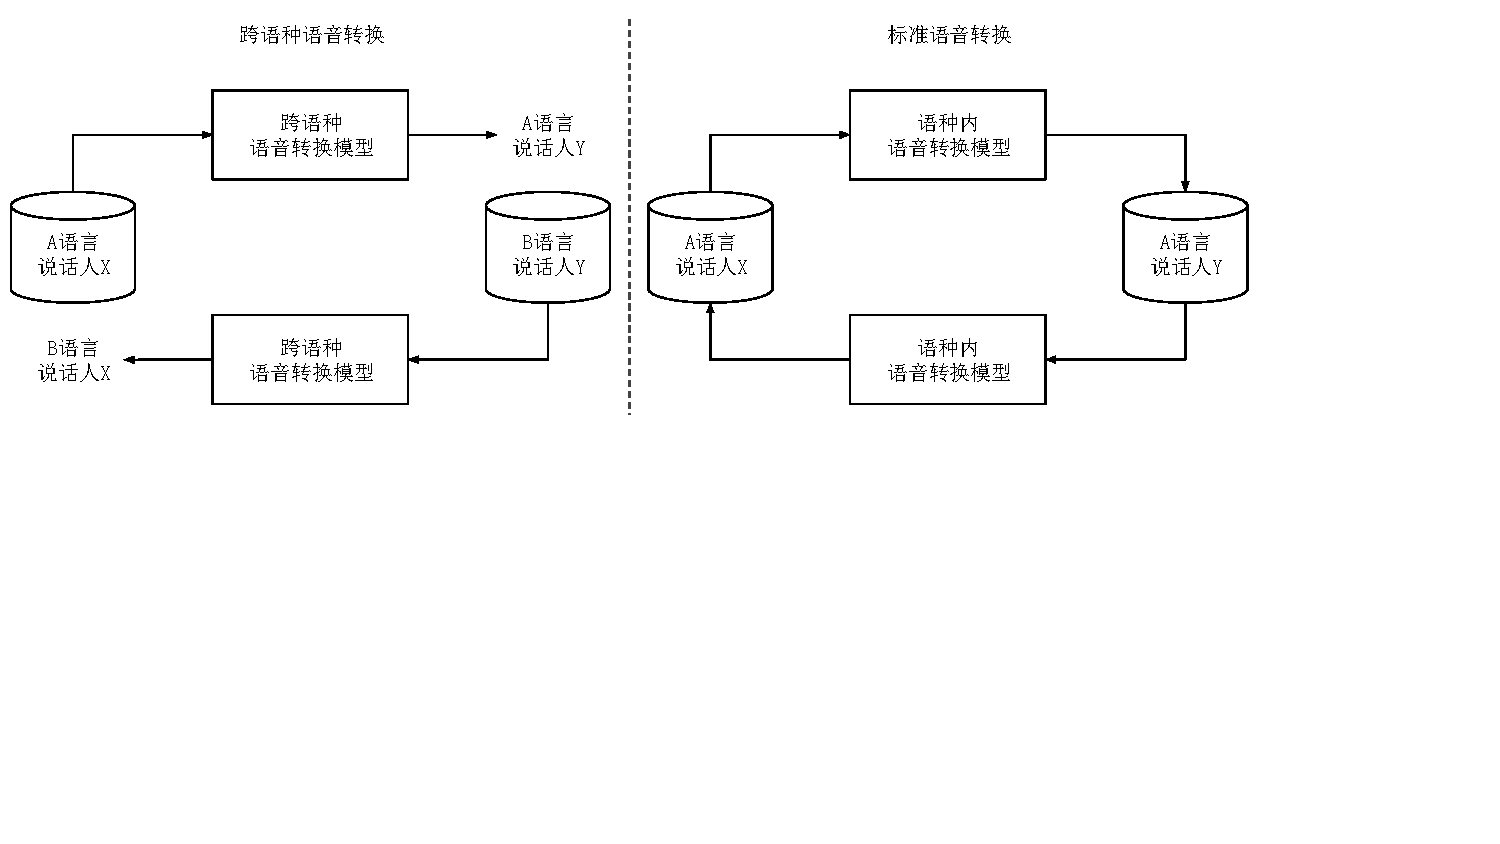
\includegraphics[width=14cm,trim=0 200 80 0,clip]{figure/5_clvc.pdf}
    \bicaption[跨语种语音转换和标准语音转换对比图]
    {跨语种语音转换和标准语音转换对比图}
    {Comparison of cross-lingual Voice Conversion and standard Voice Conversion}
    \label{fig:clvc}
\end{figure}

\begin{itemize}
    \item 不同语种之间文本信息不一致导致较难匹配。由于跨语种的语音转换涉及到两种不同的语言,因此平行语料的语音转换方法将完全不适用。
    另一方面若使用非平行的对齐方法,语种之间的巨大差异也会导致对齐准确度的下降。因此如何找到有效的单元匹配方式或无监督的训练方式是
    跨语种语音转换面临的主要挑战。
    \item 差异较大的声学特征与CycleGAN训练机制的矛盾。该矛盾分为两个方面。如前文所述,CycleGAN之所以能够实现语音转换任务,判别器在其中有着关键的作用。
    判别器在训练时,会分别输入正例和负例,对应训练标签$1$和$0$,其中正例是目标说话人的真实特征序列,负例是从原始说话人声学特征经
    生成器转换的目标说话人的转换特征序列,判别器的目标是尽可能地区分正例和负例。生成器在训练时会将生成的目标说话人转换特征传递给判别器,
    并将判别器的判别结果与$1$计算损失,来衡量转换特征和真实目标特征之间的差距,然后将梯度回传给生成器,这样生成器下次在遇到类似输入时,
    就会生成更接近判别器正例的转换特征。从图\ref{fig:clvc}中可以注意到,在跨语种语音转换中,判别器的正例
    是目标语种的目标说话人特征序列,而负例是原始语种的目标说话人特征序列。当判别器尝试区分正负例时,总是会尝试以区分度最大的信息作为
    判别要素,此时当语种信息的差异化大于说话人信息的差异化时,判别器就会转变为一个语种分类器,进而导致生成器无法从判别器中得到正确的
    梯度,因此在基线试验中,经常会导致模型在训练时无法训练成功:输入中文,生成器会输出无意义的英文语音。另一方面,语种的差异也会导致
    跨语种语音转换没有一个标准的对偶任务。如图\ref{fig:clvc}中左图所示,主任务为将说话人X的A语言转为说话人Y的A语言,理论上对偶任务
    应是说话人Y的A语言转为说话人X的A语言,而实际上对偶任务则是说话人Y的B语言转为说话人X的B语言。这样的不完全对偶性也增加了CycleGAN在
    跨语种语音转换任务上的难度。
\end{itemize}

\section{说话人识别}
\subsection{说话人识别概述}
说话人识别,也称声纹识别,同指纹识别,人脸识别相同,是一种新兴的生物特征识别技术。该技术从连续的语音信号中提取说话人相关的离散特征,
将说话人特征与数据库中的特征进行对比,得到匹配的说话人身份,从而实现对说话人身份的识别。说话人识别技术与语音识别技术都是输入语音信号
的分类任务。但不同的是,语音识别更专注于语音的说话内容,并尽量忽视掉说话人信息,而说话人识别则更注重语音的说话人是谁,而相对较少
关注语义信息。对于不同的说话人,其声道长度,声带基频,口腔及发音习惯等都有较大的区别,因而可以根据语音来判断说话人的身份,由于不同
发音人的语速,节奏也有区别,因此韵律信息也会被考虑。说话人识别通用框架主要包括两个部分,注册以及测试。注册是指用需要识别的说话人语音训练
识别模型,测试则是用训练好的模型对新来的语音进行识别。

根据实际应用场景的不同,说话人识别可以分为两类:说话人确认(Speaker Verification)和说话人辨认(Speaker Identification)。
其中说话人确认是针对某个特定说话人的识别,对于输入的语音,说话人确认模型输出是/否,代表该语音是否是该说话人
所说,属于二分类问题。说话人辨认则是对于输入的语音,在给定的说话人集合中,找出最符合的一个说话人,输出该语音是哪个说话人所说,
是多分类问题。说话人识别和说话人辨认主要在训练数据和输出层面有所区别,相比而言,说话人辨认在候选集合较大时,难度较高。
根据注册和测试时语音文本是否一致,可以将说话人识别分为文本相关(Text-dependent)的识别和文本无关(Text-independent)的说话人识别。
文本相关的说话人识别要求测试时提供的语音文本内容与训练时相同,模型在文本相同的先验下判断说话人身份,往往可以达到不错的性能。而文本无关的说话人识别则对
测试时的文本内容没有限制,使用环境也相对更自由,但建模难度也往往更大。说话人识别的应用非常广泛,包括声纹加密,语音检索,说话人核对,
和司法鉴定等。

在2012年以前,说话人识别的研究还主要以基于统计的机器学习方法为主,在2012年后以深度学习为基础的方法不断提出,如bottleneck feature、
d-vector、x-vector和j-vector等,一些最新的思想也被加入训练过程中,如基于注意力机制和learning to rank的算法等。
可以这些算法分为三类:基于i-vector的算法,基于DNN的算法和基于注意力机制和learning to rank等的改良算法。
其中基于DNN的算法中,早期用DNN以替代GMM计算后验概率,2014年Google提出的d-vector为标志\cite{variani2014deep},后续提出了一系列基于DNN的方法如
x-vector,j-vector等\cite{snyder2016deep,chen2015multi,shi2017double}。本文将采用基于d-vector的说话人识别技术,
将其应用到跨语种语音转换中。

\subsection{d-vector说话人特征}

\begin{figure}[!htp]
    \centering
    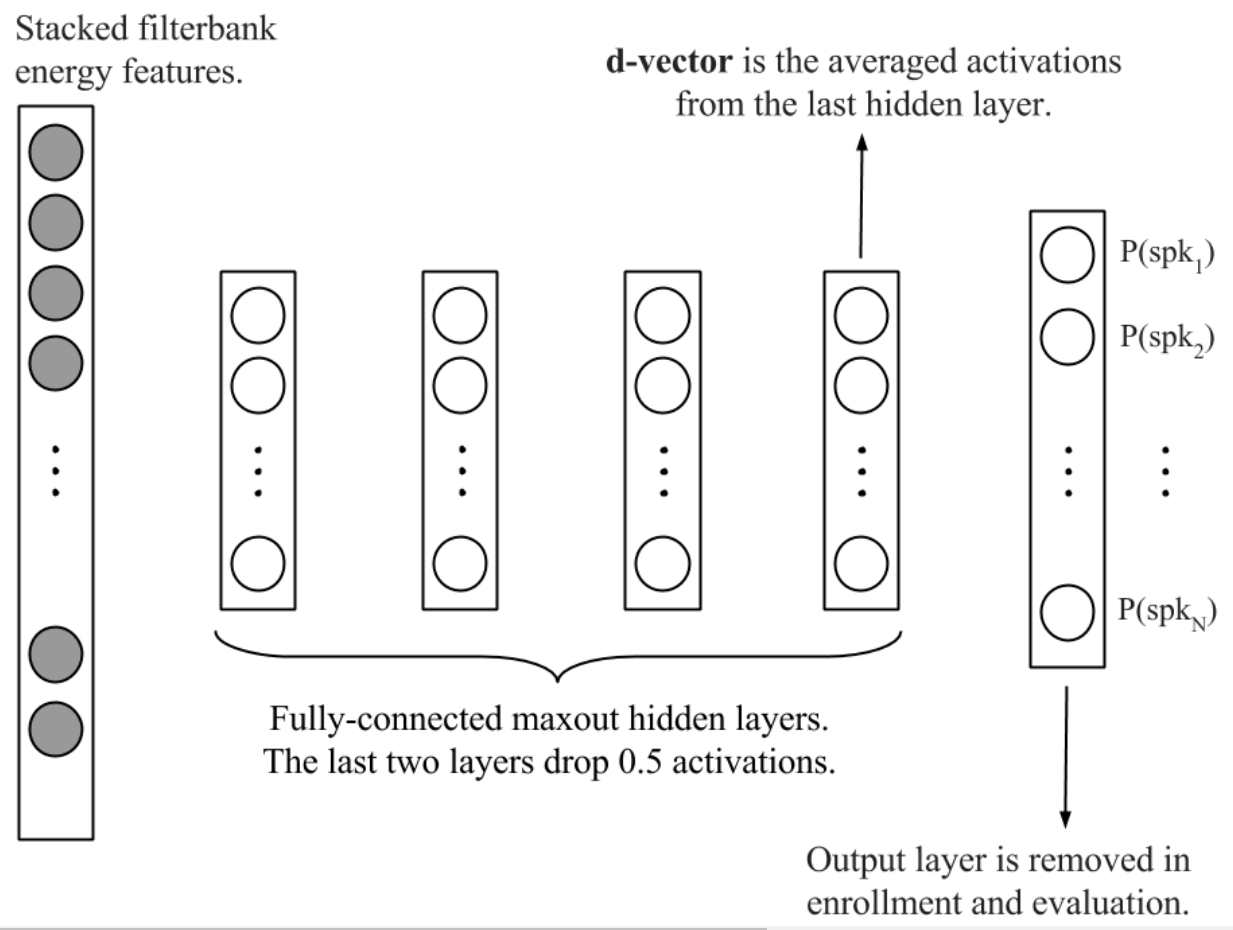
\includegraphics[width=12cm,trim=0 10 0 0,clip]{figure/5_dvector.png}
    \bicaption[基于DNN的说话人验证示意图\cite{variani2014deep}]
    {基于DNN的说话人验证示意图\cite{variani2014deep}}
    {Schematic diagram of the DNN model for speaker verification}
    \label{fig:dvector}
\end{figure}

基于d-vector的说话人特征提取模型如图~\ref{fig:dvector}如图所示。该方法和核心在于使用DNN网络作为一个说话人
特征提取器。在该目标下,首先在帧级别训练一个有监督的DNN模型。模型的输入是动态声学特征,即当前帧和前后若干帧的
拼接,目的是希望模型在判断时同时考虑一定范围内的上下文信息。模型的输出是一个向量,向量的长度取决于说话人的个数$N$。
训练时目标标签则是长度为$N$的one-hot向量,即除了输入特征对应的说话人序号在向量中的位置为1,其他值皆为0。

当DNN说话人识别模型训练完成后,即将DNN模型最后一个隐层的激励函数输出作为一个新的说话人表示(d-vector)。对于一句新的语音,
DNN对其中的每一帧都可以得到一个隐层向量,将所有帧的隐层向量累积起来,得到最终的说话人表示。这里选用最后一个隐层
的激励函数输出作为说话人表示而不是最终的$softmax$层,是因为输出层的长度是依赖于训练的说话人总数,无法根据具体
需要改变长短,而最后一个隐层则可以做到这点;另一方面,作者在实验中也发现最后一层隐层向量相比最终输出,其在没有见过
的说话人上有着更好的泛化性。d-vector的假设是认为训练好的DNN说话人识别模型,已经在最后一个隐层中学到了较为紧凑的说话人
表示,当训练时的说话人数目较多时,该表示也可以用来表达没有见过的说话人。

在测试阶段,给定一个特定说话人$s$的语音句集合$X_s = \left\{O_{s_{1}},O_{s_{2}},...,O_{s_{n}}\right\}$。
其中每个句子是一个观测集合$O_{s_{i}} = \left\{O_1,o_2,...,o_m\right\}$。首先对于每个观测,通过拼接上下帧得到其
动态特征,输入给训练好的DNN模型,获得对应的最后一层隐层向量输出,并将其归一化,作为该帧的d-vector。最终说话人$s$的表示则
是通过将所有的d-vector进行平均得到。当得到该说话人的一个新的语句时,将该句的d-vector与之前得到的说话人的最终表示计算
余弦距离,通过一个预先设定的阈值来得到最终的识别结果。

\section{引入说话人特征的跨语种语音转换}

\begin{figure}[!htp]
    \centering
    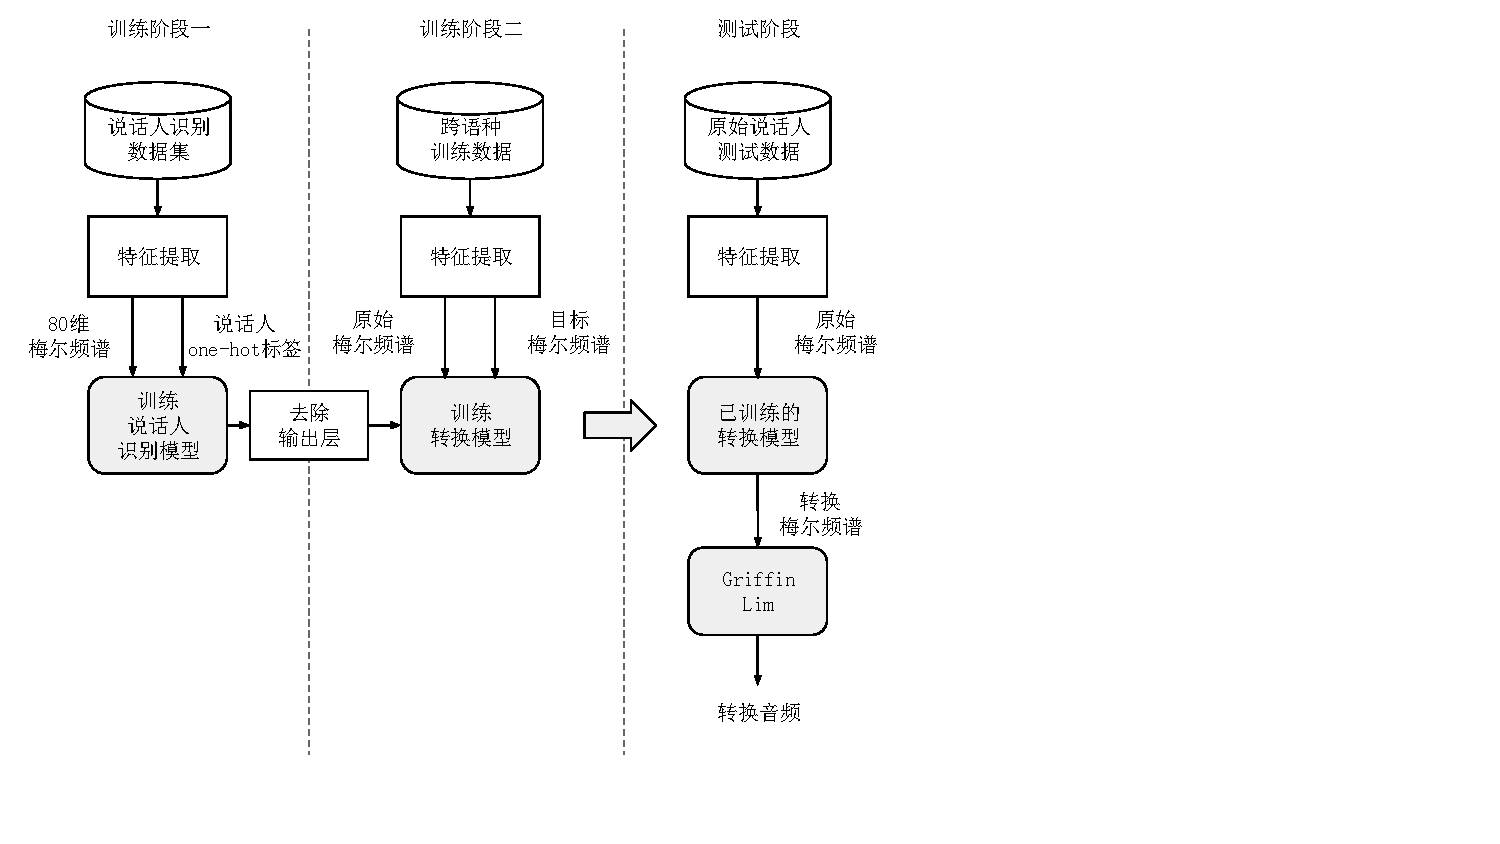
\includegraphics[width=12cm,trim=0 50 250 0,clip]{figure/5_proposedarch.pdf}
    \bicaption[引入d-vector的语音转换示意图]
    {引入d-vector的语音转换示意图}
    {Schematic diagram of the d-vector based Voice Conversion}
    \label{fig:5proposedarch}
\end{figure}

如图~\ref{fig:5proposedarch}所示,引入d-vector的跨语种语音转换方法分为三个阶段。在训练阶段一,一个语种无关的说话人识别模型在
专门用于说话人识别的数据集上进行训练,由于说话人识别模型将接入转换模型训练,为了与转换模型保持一致,
这里使用80维的梅尔频谱,并将对应的标签改为说话人的one-hot向量;在训练阶段二,将训练好的说话人识别模型去除输出层后,
作为说话人特征提取器加入转换模型中,在跨语种的语音转换数据集上进行特征提取和训练;测试阶段同通常的语音转换相同,先对测试的原始
语音提取特征,并传递给训练好的转换模型,得到模型输出的转换特征后使用Griffin Lim算法生成声音。
下文将详细介绍本文使用的语种无关的d-vector提取器和其与CycleGAN转换模型的结合。



\subsection{d-vector提取器和CycleGAN的结合}

\begin{figure}[!htp]
    \centering
    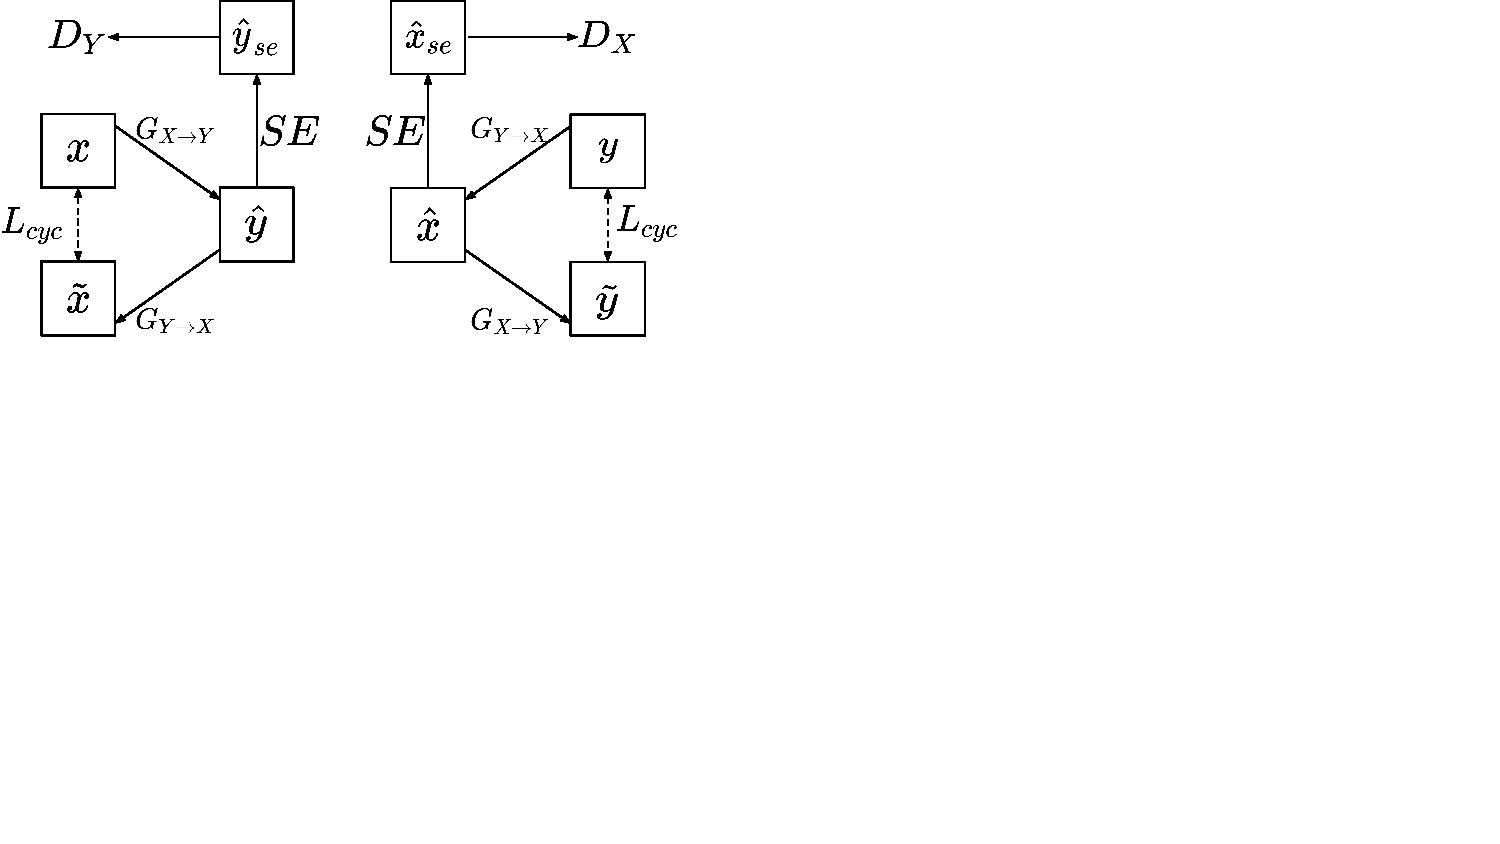
\includegraphics[width=10cm,trim=0 220 370 0,clip]{figure/5_dvectorcyclegan.pdf}
    \bicaption[基于d-vector提取器的CycleGAN模型示意图]
    {基于d-vector提取器的CycleGAN模型示意图}
    {Schematic diagram of the d-vector extractor based CycleGAN}
    \label{fig:dvectorcyclegan}
\end{figure}

如前文所述,跨语种的一大难点是差异较大的声学特征与CycleGAN训练机制的矛盾,其中主要矛盾是在CycleGAN模型
的训练过程中,判别器的正例和负例不仅在说话人信息上具有差异,由于语种的不同,在语义信息上也有着巨大的差异,
因此当语义信息的差异大于说话人信息的差异时,模型就会由说话人区分器变为语种区分器,极大降低了模型性能。
本章因此提出的引入说话人信息的语音转换方法,转换模型结构如图~\ref{fig:dvectorcyclegan}所示,其中$SE$
代表d-vector提取器,由预先训练好的语种无关的说话人分类器去掉输出层得到,$\hat{y}_{se}$是指由d-vector
提取器从转换特征和真实特征提取出的d-vector向量。可以看出,其与标准CycleGAN的最大不同是在判别器之前加入了
一个前置网络。该前置网络可以将声学特征向量中的说话人信息提取出来,进而在一定程度上忽略其中的语义信息。提取出来的
说话人表示再传递给对应的判别器,此时判别器只需要从说话人表示中判定真假,而可以在较大程度上减少语种信息对判别器的
影响。在整个模型的训练过程中,d-vector提取器只需要预先训练,之后就将参数固定,不再更新参数,只需要前向传播和
反向计算梯度,将判别器的梯度传递给生成器即可。此时对抗损失变为

\begin{align}
    L_{adv}(G_{X\rightarrow Y},D_Y) & =\mathbb{E}_{y\sim P_{Data}(y)}\left[log D_Y(SE(y))\right] \\
    & + \mathbb{E}_{x\sim P_{Data}(x)}\left[log(1-D_Y(SE(G_{X\rightarrow Y}(x))))\right] \\
    L_{adv}(G_{Y\rightarrow X},D_X) & =\mathbb{E}_{x\sim P_{Data}(x)}\left[log D_X(SE(x))\right] \\
    & + \mathbb{E}_{y\sim P_{Data}(y)}\left[log(1-D_X(SE(G_{Y\rightarrow X}(y))))\right]
\end{align}

$SE$在其中可以看成一个可以前向和反向传播的过滤模型,该模型输入声学特征,将其中的说话人之外的信息过滤掉,只留下
其中的说话人信息。这样判别器就可以在跨语种的数据集上实现类似同语种转换的效果。



\subsection{语种无关的d-vector提取器训练}


\begin{figure}[!htp]
    \centering
    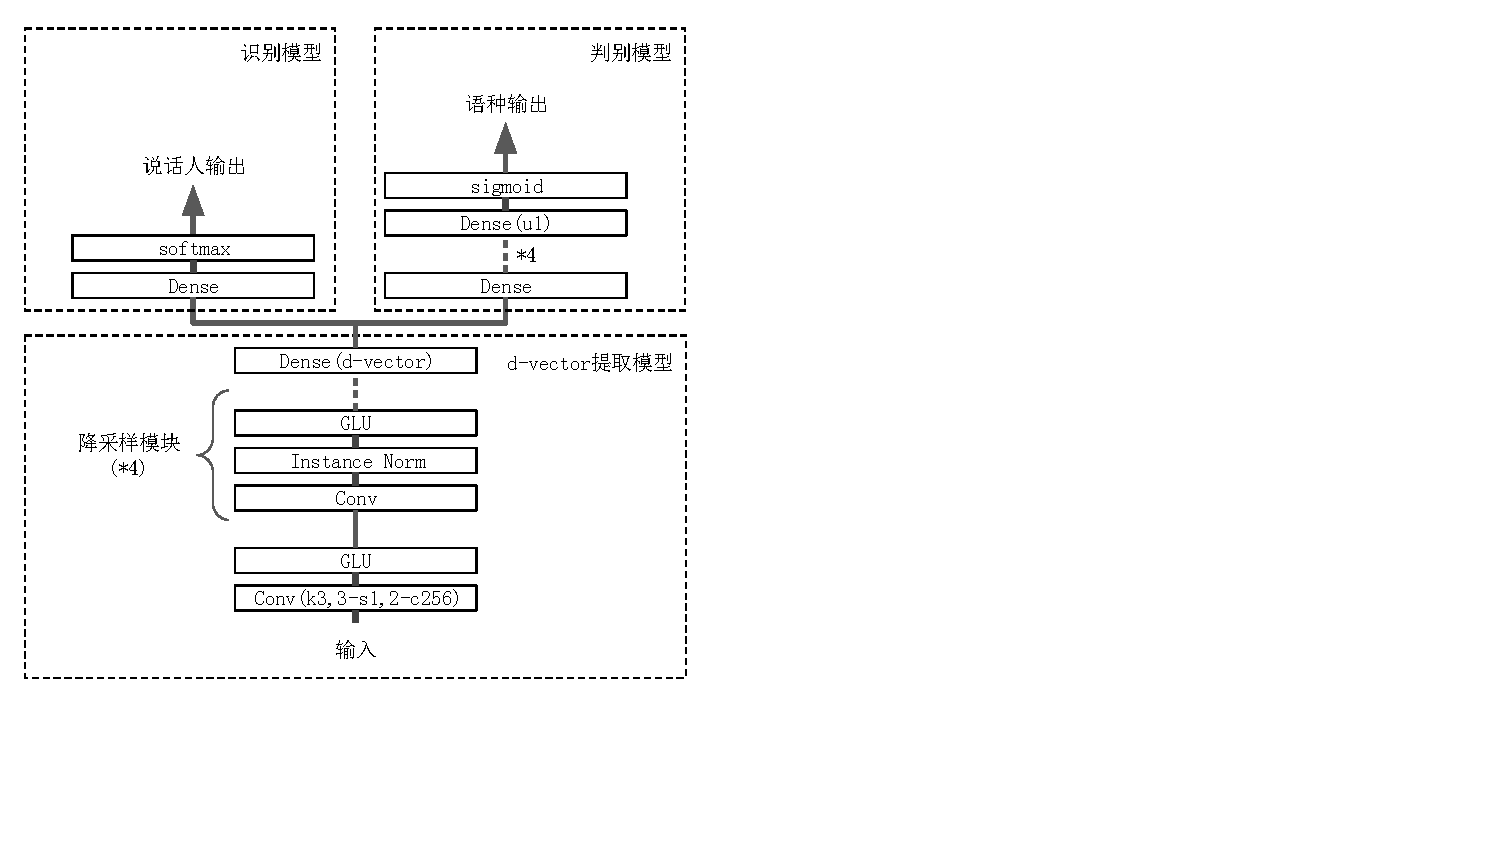
\includegraphics[width=12cm,trim=0 79 380 0,clip]{figure/5_d.pdf}
    \bicaption[说话人识别模型网络结构图]
    {说话人识别模型网络结构图}
    {Architecture of the speaker verification networks}
    \label{fig:5d}
\end{figure}

d-vector提取器作为判别器的前置网络,其功能从输入的声学特征序列中提取说话人表示,并尽可能地过滤掉特征中的语义语种信息。
对于训练一个标准的d-vector提取器来说,通常首先需要较多说话人的语料数据,每个说话人包含几句到几十句不等,目前常用的
开源数据中包括英文数据集voxceleb\cite{nagrani2017voxceleb}以及中文数据集CN-celeb\cite{fan2019cn}。不同于
通常的说话人识别任务,为了能够对原始语言的真实原始特征和目标语言的转换原始特征进行说话人信息上的判别,提取出的说话人表示
需要在中文和英文上尽可能一致,但是通常的做法并不能保证这一点。例如,使用英文数据集训练的d-vector提取器,如果测试时使用
数据集中一个说话人的中文语音,那么由于d-vector只见过英文,则提取出的说话人表示和这个说话人英文语音的表示很可能有较大差别。
即使d-vector在训练时见过两种语言,也不能认为这样训练出来的提取器不会考虑语种信息,这就陷入了同CycleGAN一样的问题。
解决该问题的方法有两种,一种是从数据角度入手,如果能够收集每个说话人都是双语或多语种说话人,可以收集到他们说不同的语种的语音
并且这样的说话人数据足够多的话,说话人识别模型则会将同一说话人的不同语种映射到同一个标签上,从而实现对语种的过滤。但这种方法通常
不可行,因为双语说话人的数据获取难度很大,更不用说很多个说话人了。因此本章提出另一种方法,即从对抗学习的角度来解决这个问题。

本章提出一种基于对抗学习的说话人识别网络结构。如图\ref{fig:5d}所示,该网络由三个部分组成,d-vector提取模型$V$,
识别模型$C$和判别模型$D$构成。其中d-vector提取模型$V$负责从输入的声学特征中提取说话人表示,然后识别模型$C$从该说话人表示中
得到对应的说话人身份,另一方面说话人表示也传递给判别模型$D$,来输出对应的语种。这里d-vector提取模型$V$和判别模型$D$是对抗训练的,
即判别模型$D$的目标是尽可能地识别出d-vector属于哪个语种,而d-vector提取模型$V$则尽可能地生成无法判断语种的d-vector来欺骗判别模型$D$。
损失函数表示如下


\begin{align}
    L_{adv}(D) & =\mathbb{E}_{x\sim P_{Data}(x)}\left[log D(V(x))\right] \\
               & +\mathbb{E}_{y\sim P_{Data}(y)}\left[1-log D(V(x))\right]\\
    L_{adv}(V) & =\mathbb{E}_{x\sim P_{Data}(x)}\left[log (0.5-D(V(x)))\right] \\
               & +\mathbb{E}_{y\sim P_{Data}(y)}\left[log (0.5-D(V(y)))\right]
\end{align}

其中$x$和$y$分别为两个语种的训练数据。这里的对抗训练可以使用两种方法,一种是如公式所示d-vector提起器目标是生成让判别器无法判断的说话人表示,
即0.5,另一种方法则是在训练d-vector提取器时对判别器的损失传递负梯度,但这样可能会让d-vector中包含相反语种的信息,因此本章使用前一种方法来
训练说话人识别模型。

\section{实验分析}
本节对本章提出的引入说话人特征的跨语种语音转换方法的模型效果进行分析,将加入d-vector的语音转换模型与
标准CycleGAN进行对比,通过主客观实验验证d-vector的有效性及不同d-vector提取器结构对转换音质的影响。
% 客观指标可以用d-vector的距离来判断
% 引入说话人特征的有效性:
% 主观实验-自然度,相似度
% 系统:
% 1. baseline, 标准CycleGAN
% 3. 加入d-vector(d-vector 64, 100人)
% 4. 加入d-vector(d-vector 64, 1000人)
% 客观实验:
% 测试接上转换特征d-vector和目标特征的差距
% 1.d-vector提取器在clvc上的区分度,[dv 64 100;dv 64 500;dv 64 1000;]
% cycle-consistency loss
\subsection{实验配置}
本章实验所使用的数据集分为两种,在训练说话人识别模型时,本章使用了中文和英文的开源数据集CN-celeb和voxceleb。其中
voxceleb是一个视听数据集,包含1251个名人的超过100,000句语音,这些语音多是从上传到Youtube的采访视频中获取的。
CN-celeb是由清华大学发布的中文说话人识别开源数据集,该数据集包含1000个名人的超过130,000句语音。在训练转换模型时,
本章所使用的数据集包括一名男性的中文说话人(lcxinm),女性的中文说话人(gpyinf)和一名女性的英文说话人(ljspeech),
音频均为录制于标准环境的标准中英口语。且训练集和测试集分别为2000句和20句,每句话长度在10s以内。
语音转换任务通常分为同性别和跨性别,因此本章将英文说话人选
为原始说话人,将中文说话人选为目标说话人,分别训练女转女的同性别转换模型和女转男的跨性别转换模型。特征提取配置参考上一章。



由于跨语种的语音转换无论在训练集还是测试集都没有平行语料,不存在真实的标签,因此很难通过频谱距离这样的客观指标来判断
特征转换的好坏。因此本章中客观实验将转换语音的d-vector与真实目标语音的d-vector进行对比来验证说话人相似度上的有效性,
同时通过转换模型训练时的重构损失来判断转换模型训练的好坏程度。
在主观实验中,本章将对自然度采用MOS打分的方式,对相似度采用ABX的偏好测试。

\subsection{客观实验}

% 1.d-vector在语音转换数据集上的分布

\begin{figure}[!ht]
    \begin{minipage}[b]{\linewidth}
        \begin{subfigure}[b]{0.33\linewidth}
            \centering
            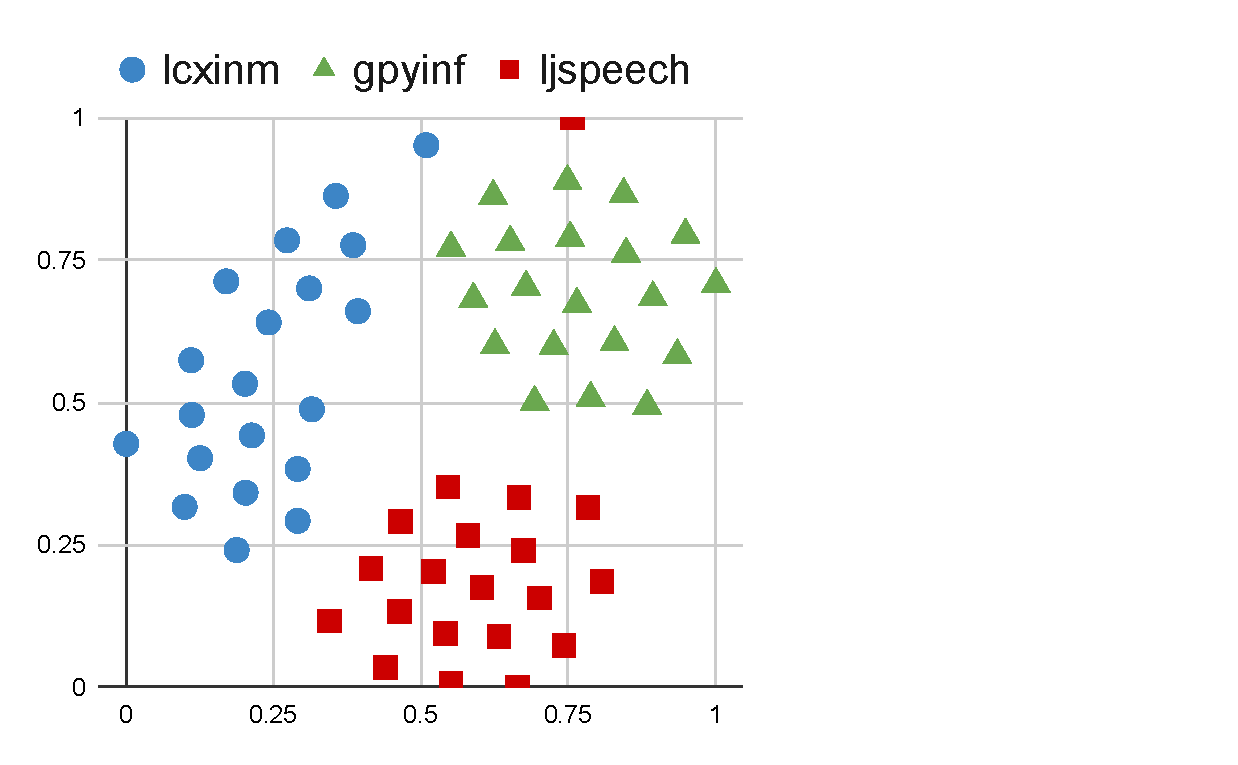
\includegraphics[width=\linewidth,trim=0 0 200 0,clip]{figure/5_dvector11.pdf}
            \caption{100 speakers w/o adv}
        \end{subfigure}        
        \begin{subfigure}[b]{0.33\linewidth}
            \centering
            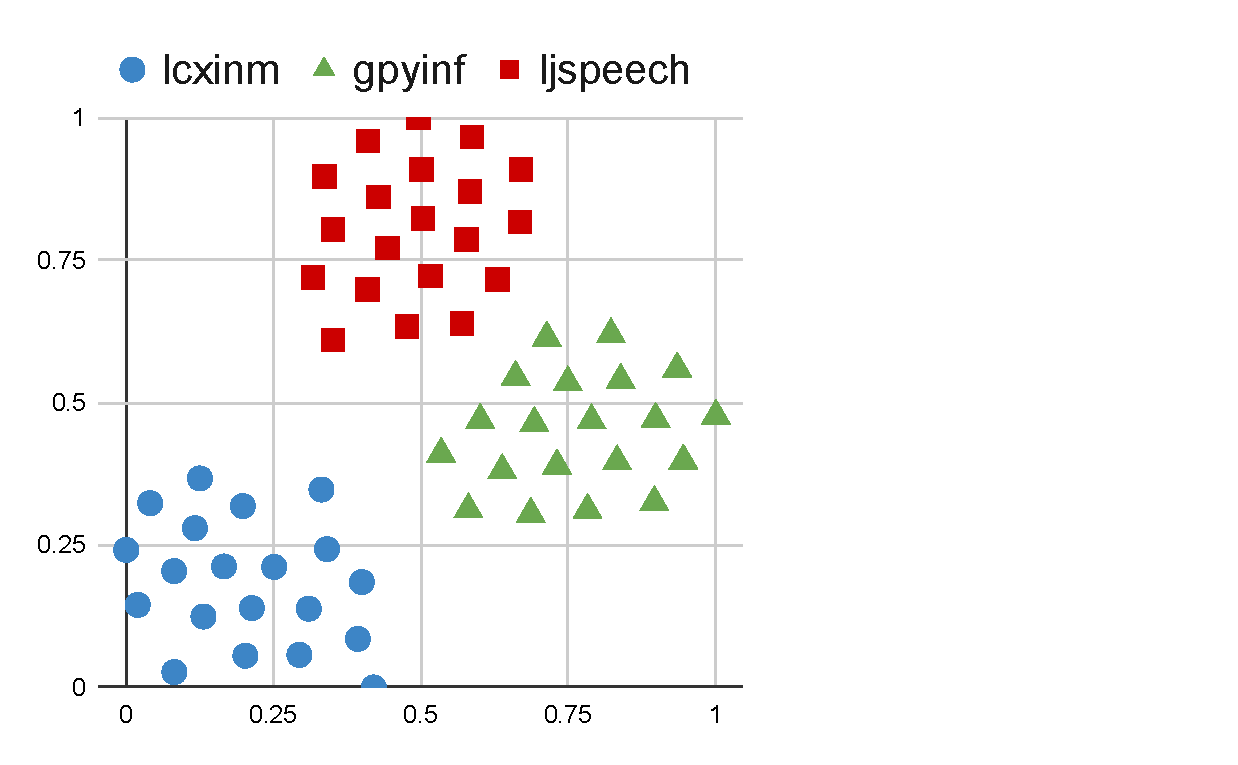
\includegraphics[width=\linewidth,trim=0 0 200 0,clip]{figure/5_dvector12.pdf}
            \caption{500 speakers w/o adv}
        \end{subfigure}   
        \begin{subfigure}[b]{0.33\linewidth}
            \centering
            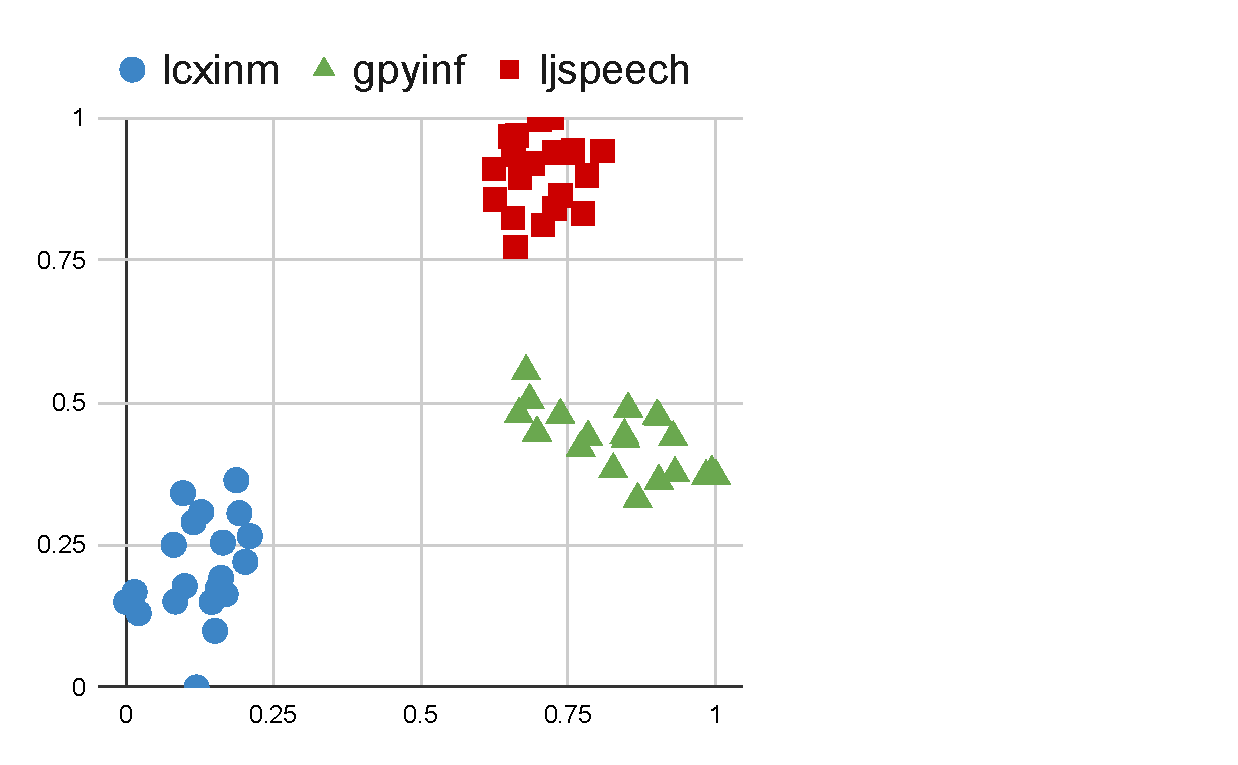
\includegraphics[width=\linewidth,trim=0 0 200 0,clip]{figure/5_dvector13.pdf}
            \caption{1000 speakers w/o adv}
        \end{subfigure}   
    \end{minipage}
    \begin{minipage}[b]{\linewidth}
        \begin{subfigure}[b]{0.33\linewidth}
            \centering
            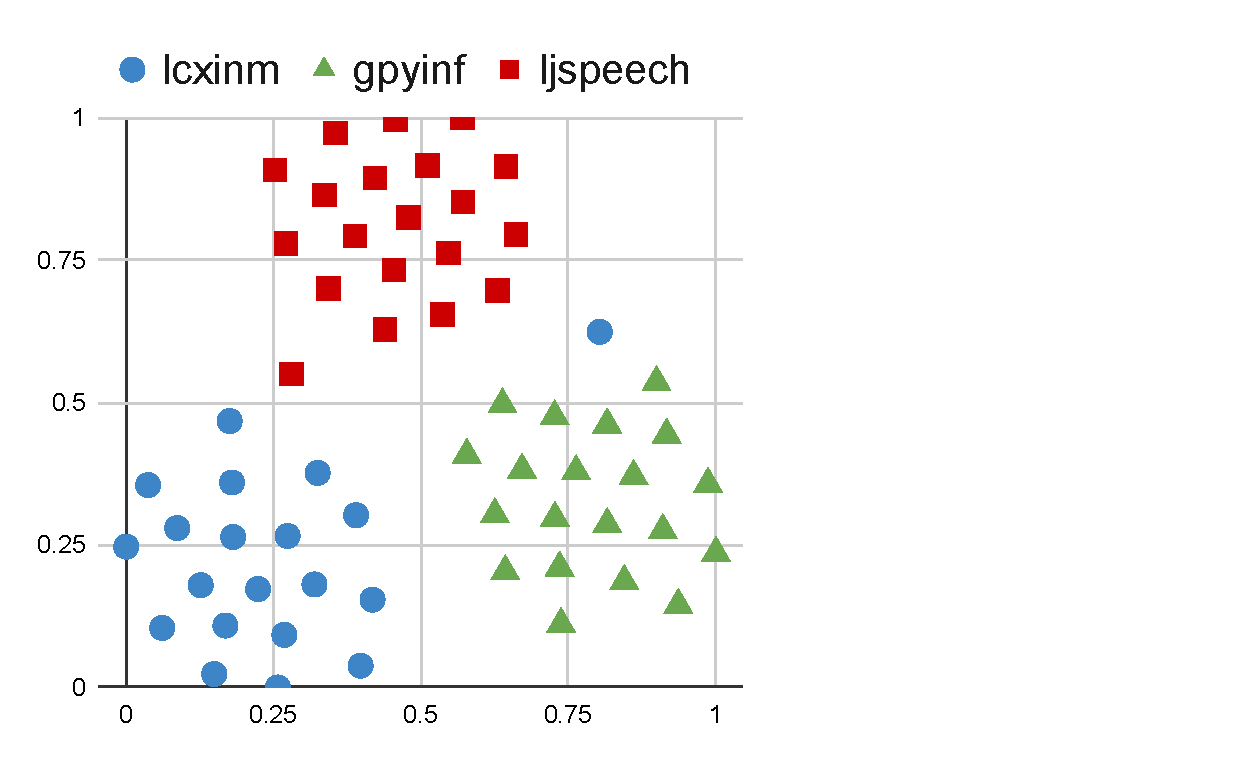
\includegraphics[width=\linewidth,trim=0 0 200 0,clip]{figure/5_dvector21.pdf}
            \caption{100 speakers w/ adv}
        \end{subfigure}        
        \begin{subfigure}[b]{0.33\linewidth}
            \centering
            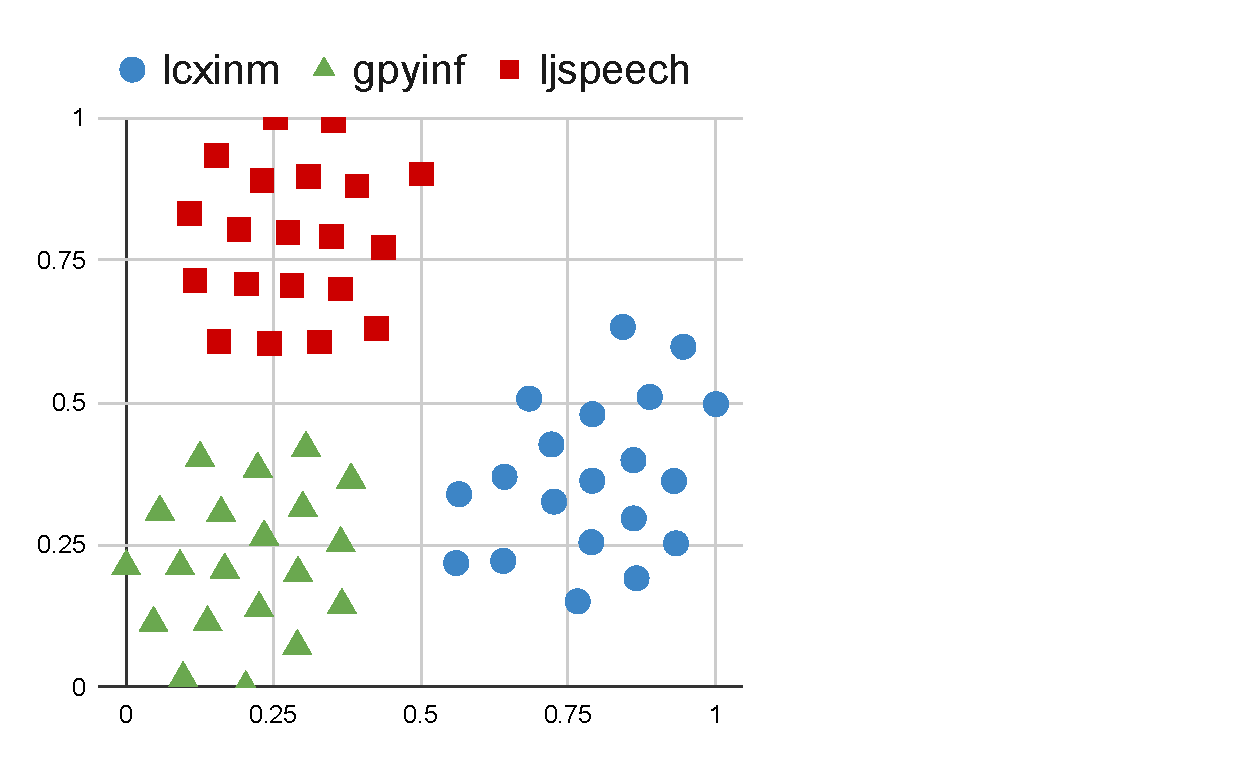
\includegraphics[width=\linewidth,trim=0 0 200 0,clip]{figure/5_dvector22.pdf}
            \caption{500 speakers w/ adv}
        \end{subfigure}   
        \begin{subfigure}[b]{0.33\linewidth}
            \centering
            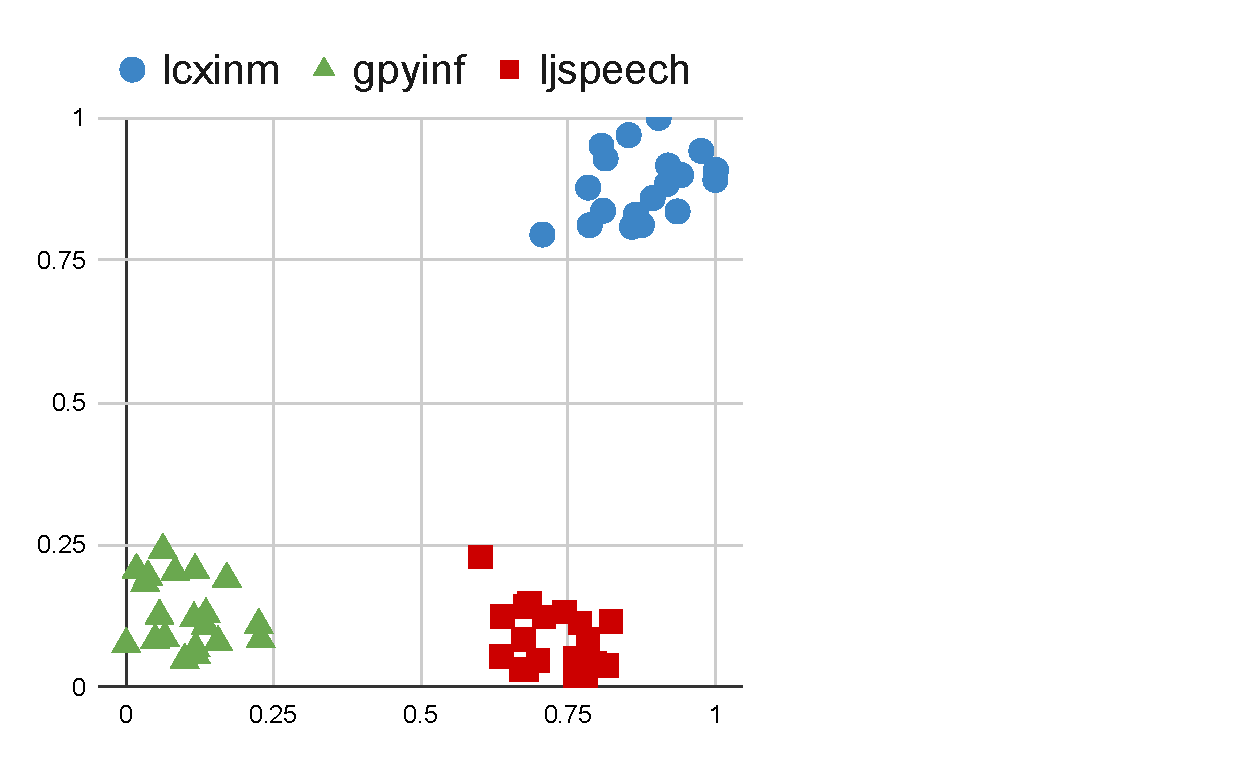
\includegraphics[width=\linewidth,trim=0 0 200 0,clip]{figure/5_dvector23.pdf}
            \caption{1000 speakers w/ adv}
        \end{subfigure}   
    \end{minipage}

    \bicaption{语音转换数据集上d-vector分布图}{Distribution of d-vector on VC corpus}
\end{figure}

% 2.d-vector的差距,使用1000句的d-vector。
% 每一组:原始;目标;baseline;没有adv;有adv
\begin{table}
    \centering
    \begin{tabular}[t]{ cccccc }
        \toprule
        % \hline
        %\multirow{1}{*}{Methods} & \multicolumn{3}{|c|}{Female to male} \\
         %\cline{2-4}
        任务  & 原始 & 目标 & CycleGAN & DV-CycleGAN & LIDV-CycleGAN  \\
         %\hline
         %\hline
        \midrule
        %\hline
        同性别    &     0.3164 &  0.0 & 0.0171 & 0.0688 & \textbf{0.0153}           \\
        %\hline
        跨性别    &    0.1533 & 0.0 & 0.1248 & \textbf{0.0506} & 0.0849  \\
        \bottomrule
        \end{tabular} 
    \bicaption{d-vector误差对比}{Female to male}
    \label{tab:f0f22}
\end{table}

% cycle-consistency loss curve
% 同性别,跨性别,
% baseline, dv, lidv
% cyclea


\begin{figure}[!ht]
    \begin{minipage}[b]{\linewidth}
        \begin{subfigure}[b]{0.48\linewidth}
            \centering
            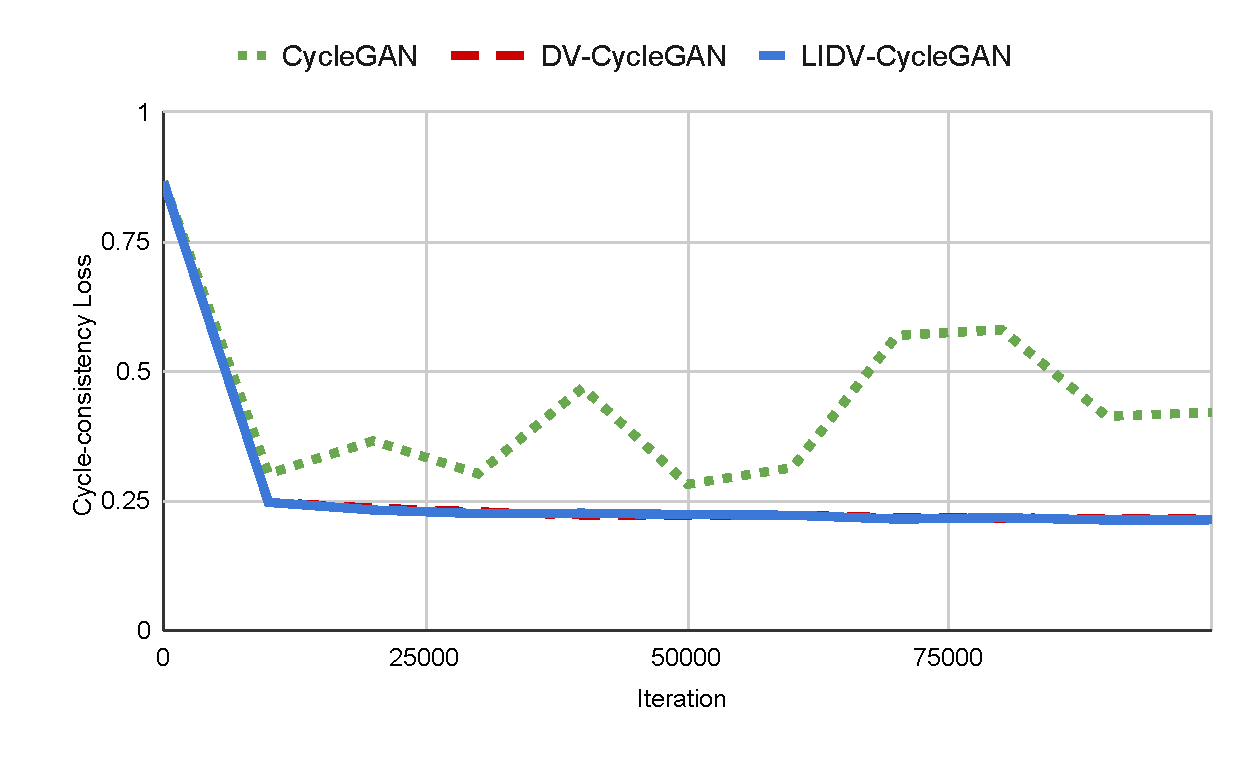
\includegraphics[width=\linewidth,trim=0 0 0 0,clip]{figure/5_cycle1.pdf}
            \caption{100 speakers w/o adv}
        \end{subfigure}        
        \begin{subfigure}[b]{0.48\linewidth}
            \centering
            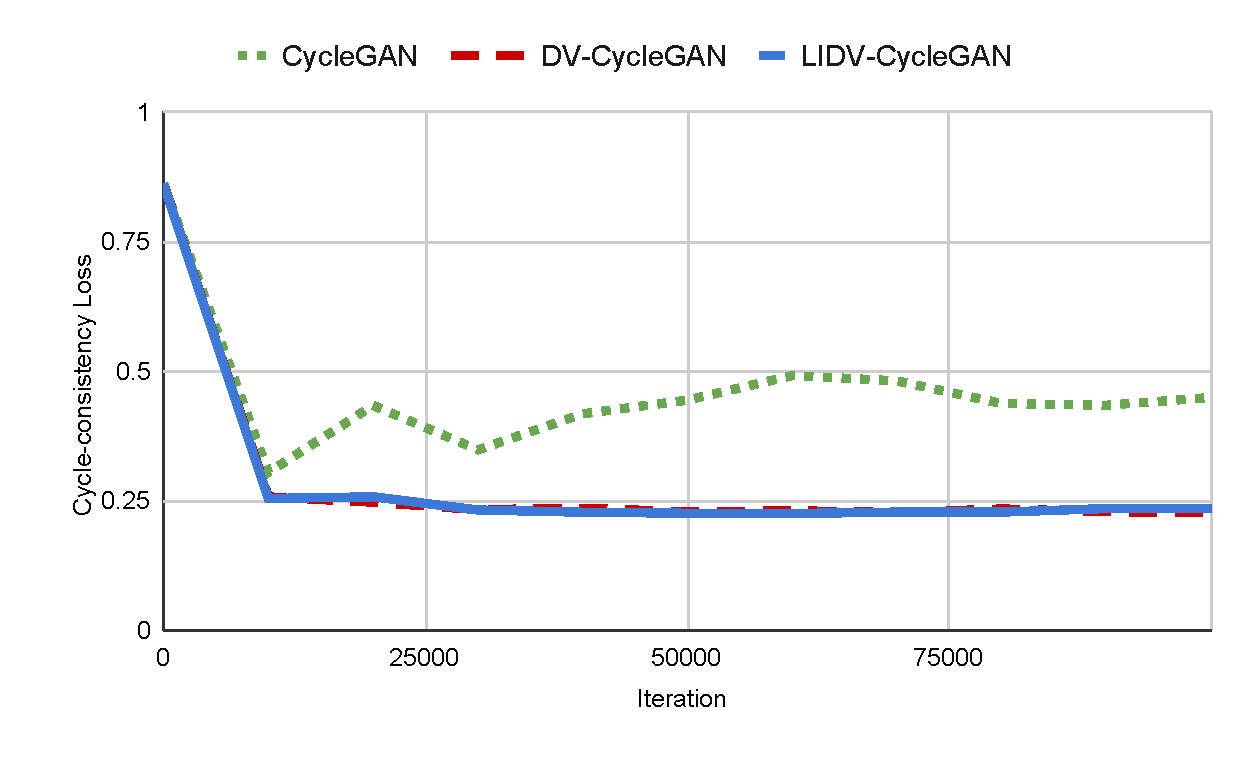
\includegraphics[width=\linewidth,trim=0 0 0 0,clip]{figure/5_cycle2.pdf}
            \caption{500 speakers w/o adv}
        \end{subfigure}   
    \end{minipage}
    \bicaption{语音转换数据集上d-vector分布图}{Distribution of d-vector on VC corpus}
\end{figure}


\subsection{主观实验}

\section{本章小结}